\chapter{NNQS exploration}\label{nnqsresults}
This chapter explores the effects of different architectures and training schemes that can be used to train NNQS to solve QUBO problems. All experiments in this section were run on a subset of the entire dataset with problem sizes of $10,25,50,75,200,250$ and $10$ problems for each problem type and size. The problem evaluation metrics are also calculated by considering the solutions from the different types of NNQS to draw a clearer comparison between architectures and training schemes.

\section{Architectures and training algorithms}
We will utilise the Restricted Boltzmann Machine (RBM) and the Multilayer Perceptron (MLP) as the architecture for NNQS. For a given input problem with $n$ variables, the RBM model will have $n$ visible nodes and $5n$ hidden nodes, while the MLP will have $n$ input nodes, $1$ hidden layer of size $5n$ and $1$ positive real output node. The RBM uses the sigmoid function, while the MLP uses the ReLU activation function. We use Gibbs sampling for the RBM and Metropolis-Hasting sampling for the MLP; both sampling methods are detailed in \autoref{samplingmethods}.

We will also compare three training algorithms for NNQS---progressive, direct, and continuous. The progressive training algorithm follows \autoref{alg:progressive}. In direct training, described in \autoref{alg:direct}, the normalised anneal fraction $s$ is held constant at $1$ for all epochs. In continuous training, described in \autoref{alg:continuous}, the normalised anneal fraction is increased gradually every epoch and the NNQS is not trained to convergence.

\begin{algorithm}
    \begin{algorithmic}
    \Require Problem Hamiltonian $\hat{H}_c$
    \Ensure Trained NNQS
    \State Initialize NNQS with random weights;
    \State Set $H \leftarrow B(1)\hat{H}_c$;
    \State Train NNQS on $H$ until convergence or until epoch limit of $1000$ is reached;
    \end{algorithmic}
    \caption{NNQS Direct Training}
    \label{alg:direct}
\end{algorithm}

\begin{algorithm}
    \begin{algorithmic}
    \Require Problem Hamiltonian $\hat{H}_c$
    \Ensure Trained NNQS
    \State Initialize NNQS with random weights;
    \For {$s \in [0.001, 1.0]$ step $0.001$}
    \State Set $H(s) \leftarrow A(s)\hat{H}_0 + B(s)\hat{H}_c$;
    \State Train NNQS on $H(s)$ for $1$ epoch;
    \EndFor
    \end{algorithmic}
    \caption{NNQS Continuous Training}
    \label{alg:continuous}
\end{algorithm}

Direct training serves as a baseline for directly training a neural network with the cost function as the problem Hamiltonian. Progressive training most closely resembles the quantum annealing process, where the system is kept at the ground state by training until convergence in each increment of $s$. Continuous training combines the other two by slowly incrementing $s$ but never reaching convergence.

\section{Results and Discussion}
Performance is shown for each dataset, accompanied by error bars representing each data point's unbiased standard error of the mean. Graphs with problem sizes on the x-axis are plotted with a log scale. The graphs for performance by size are shown in \autoref{appendix:nnqssizegraph}.

\subsection{NAE3SAT}

\begin{figure}[!htbp]
    \centering
    \subfloat[Normalized energy]{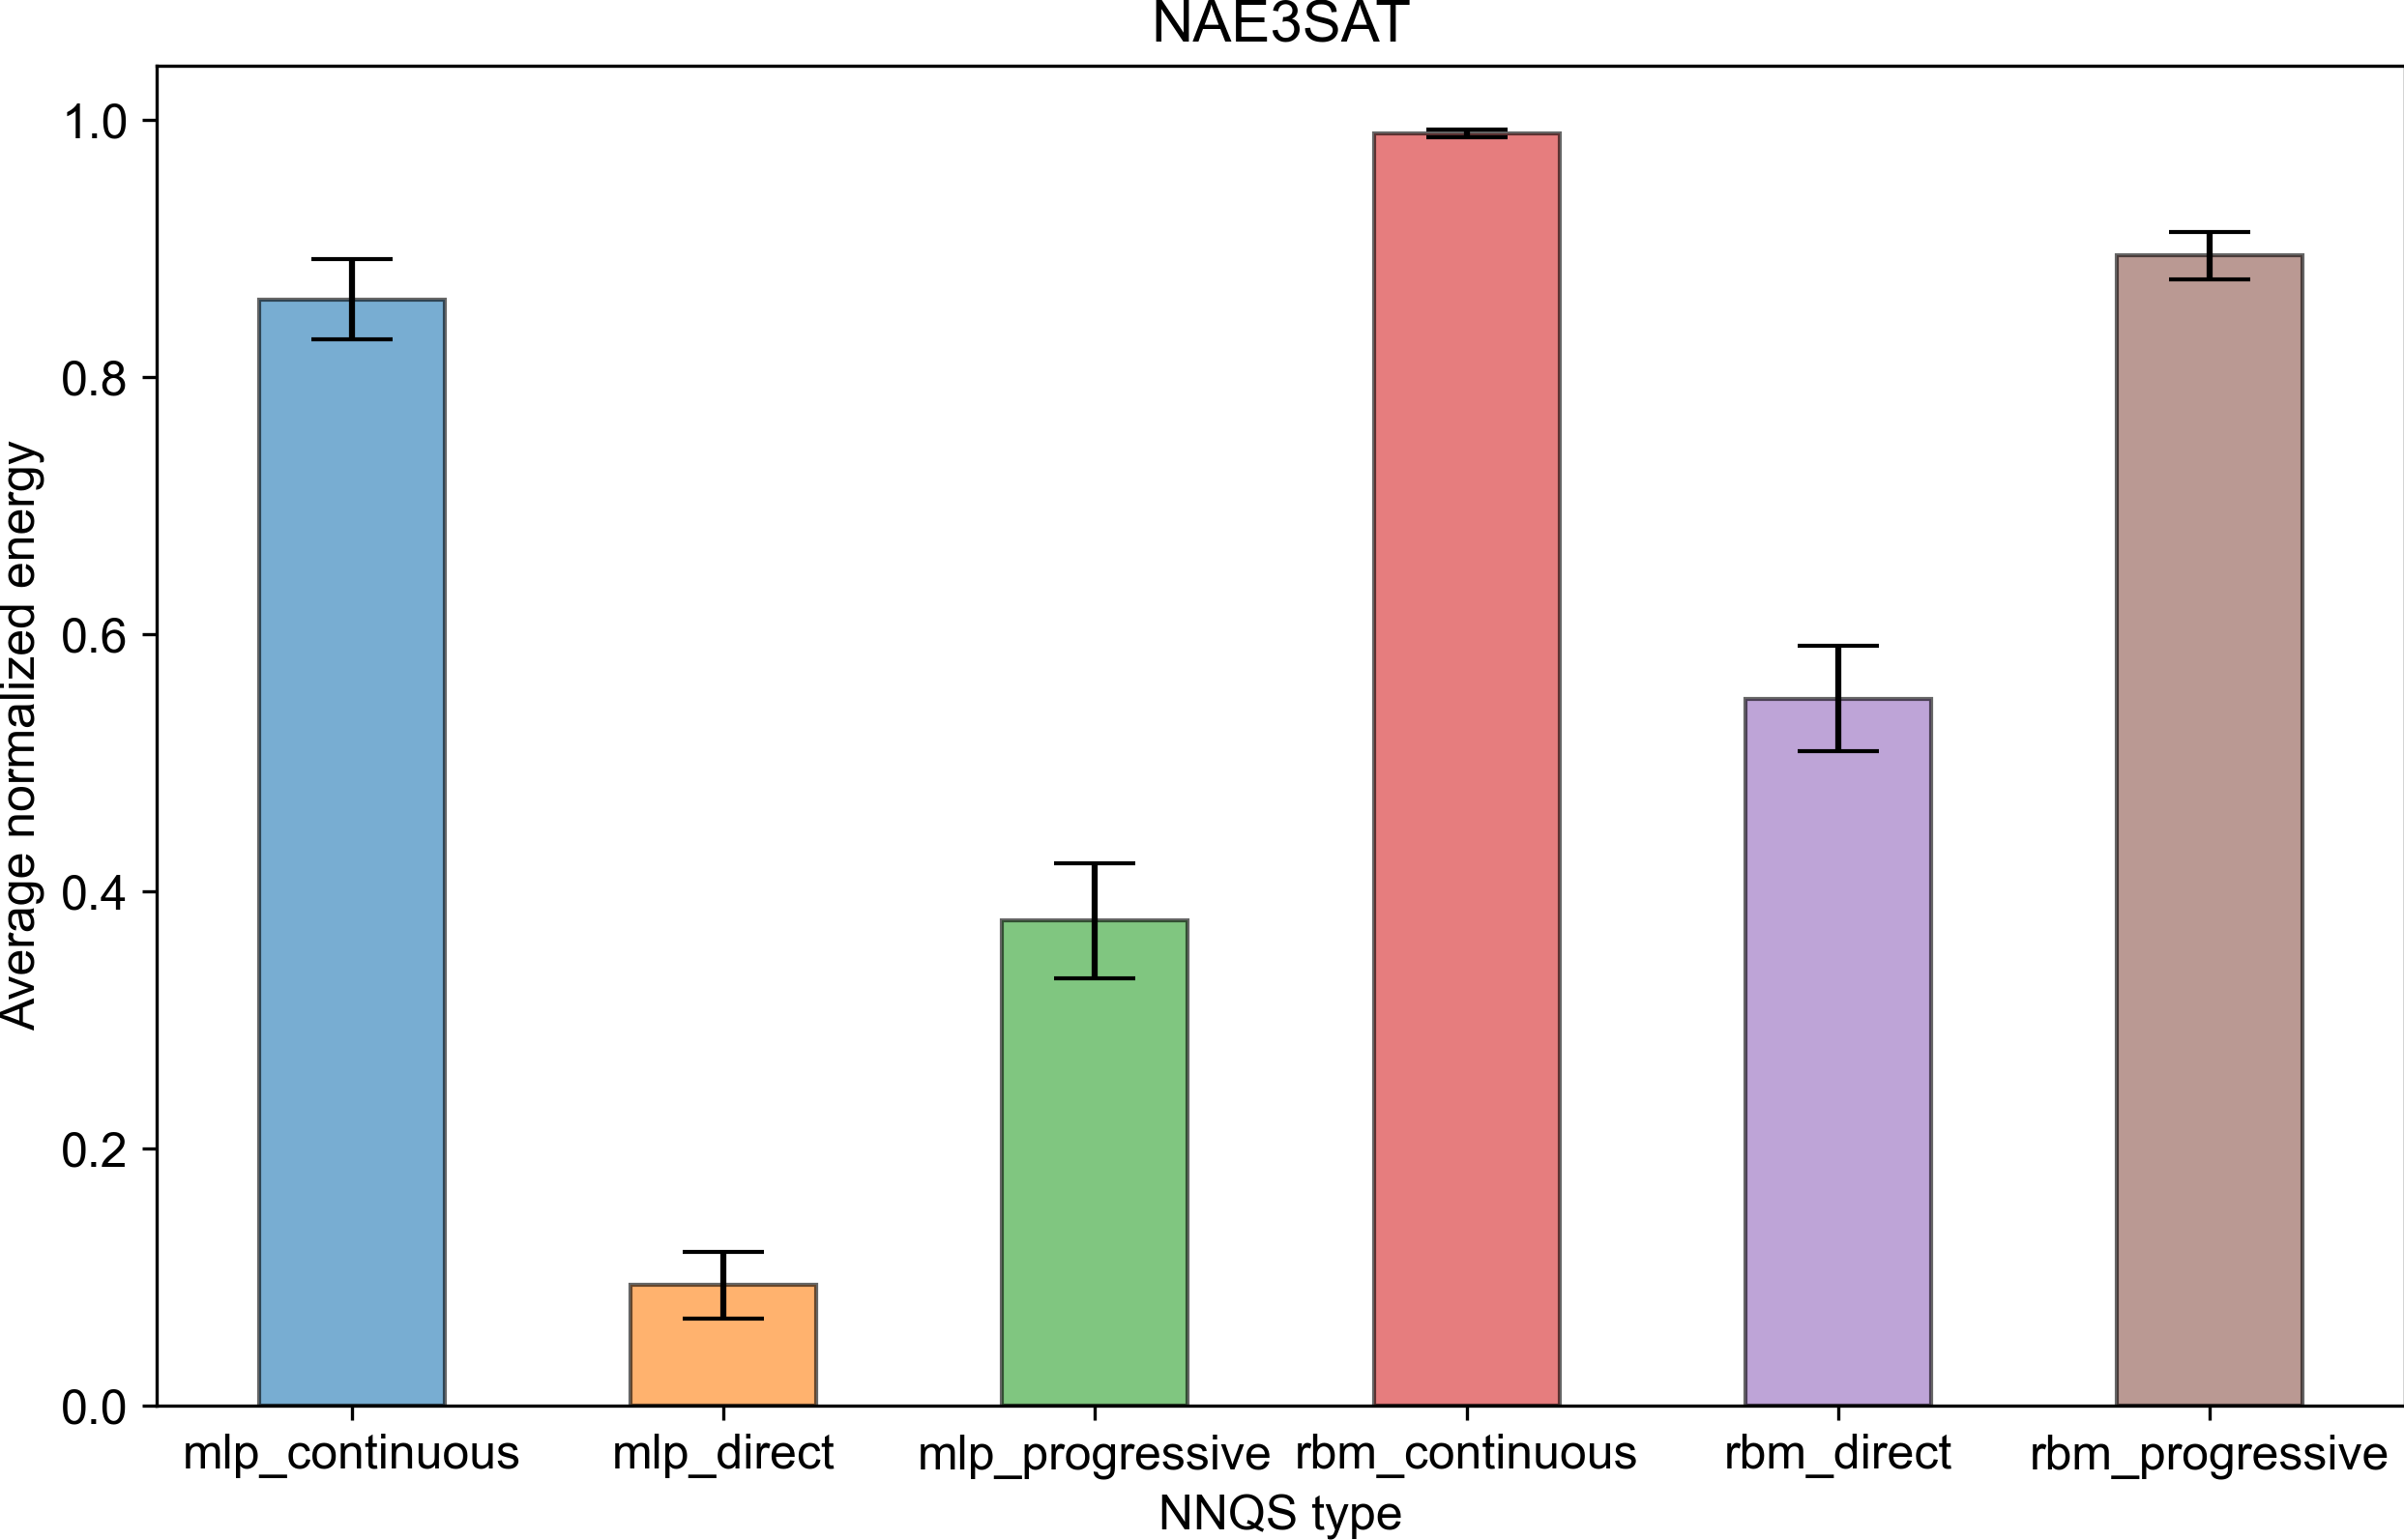
\includegraphics[width=0.49\textwidth]{images/nae3sat_nnqs_avg.png}}\hfill
    \subfloat[Success probability]{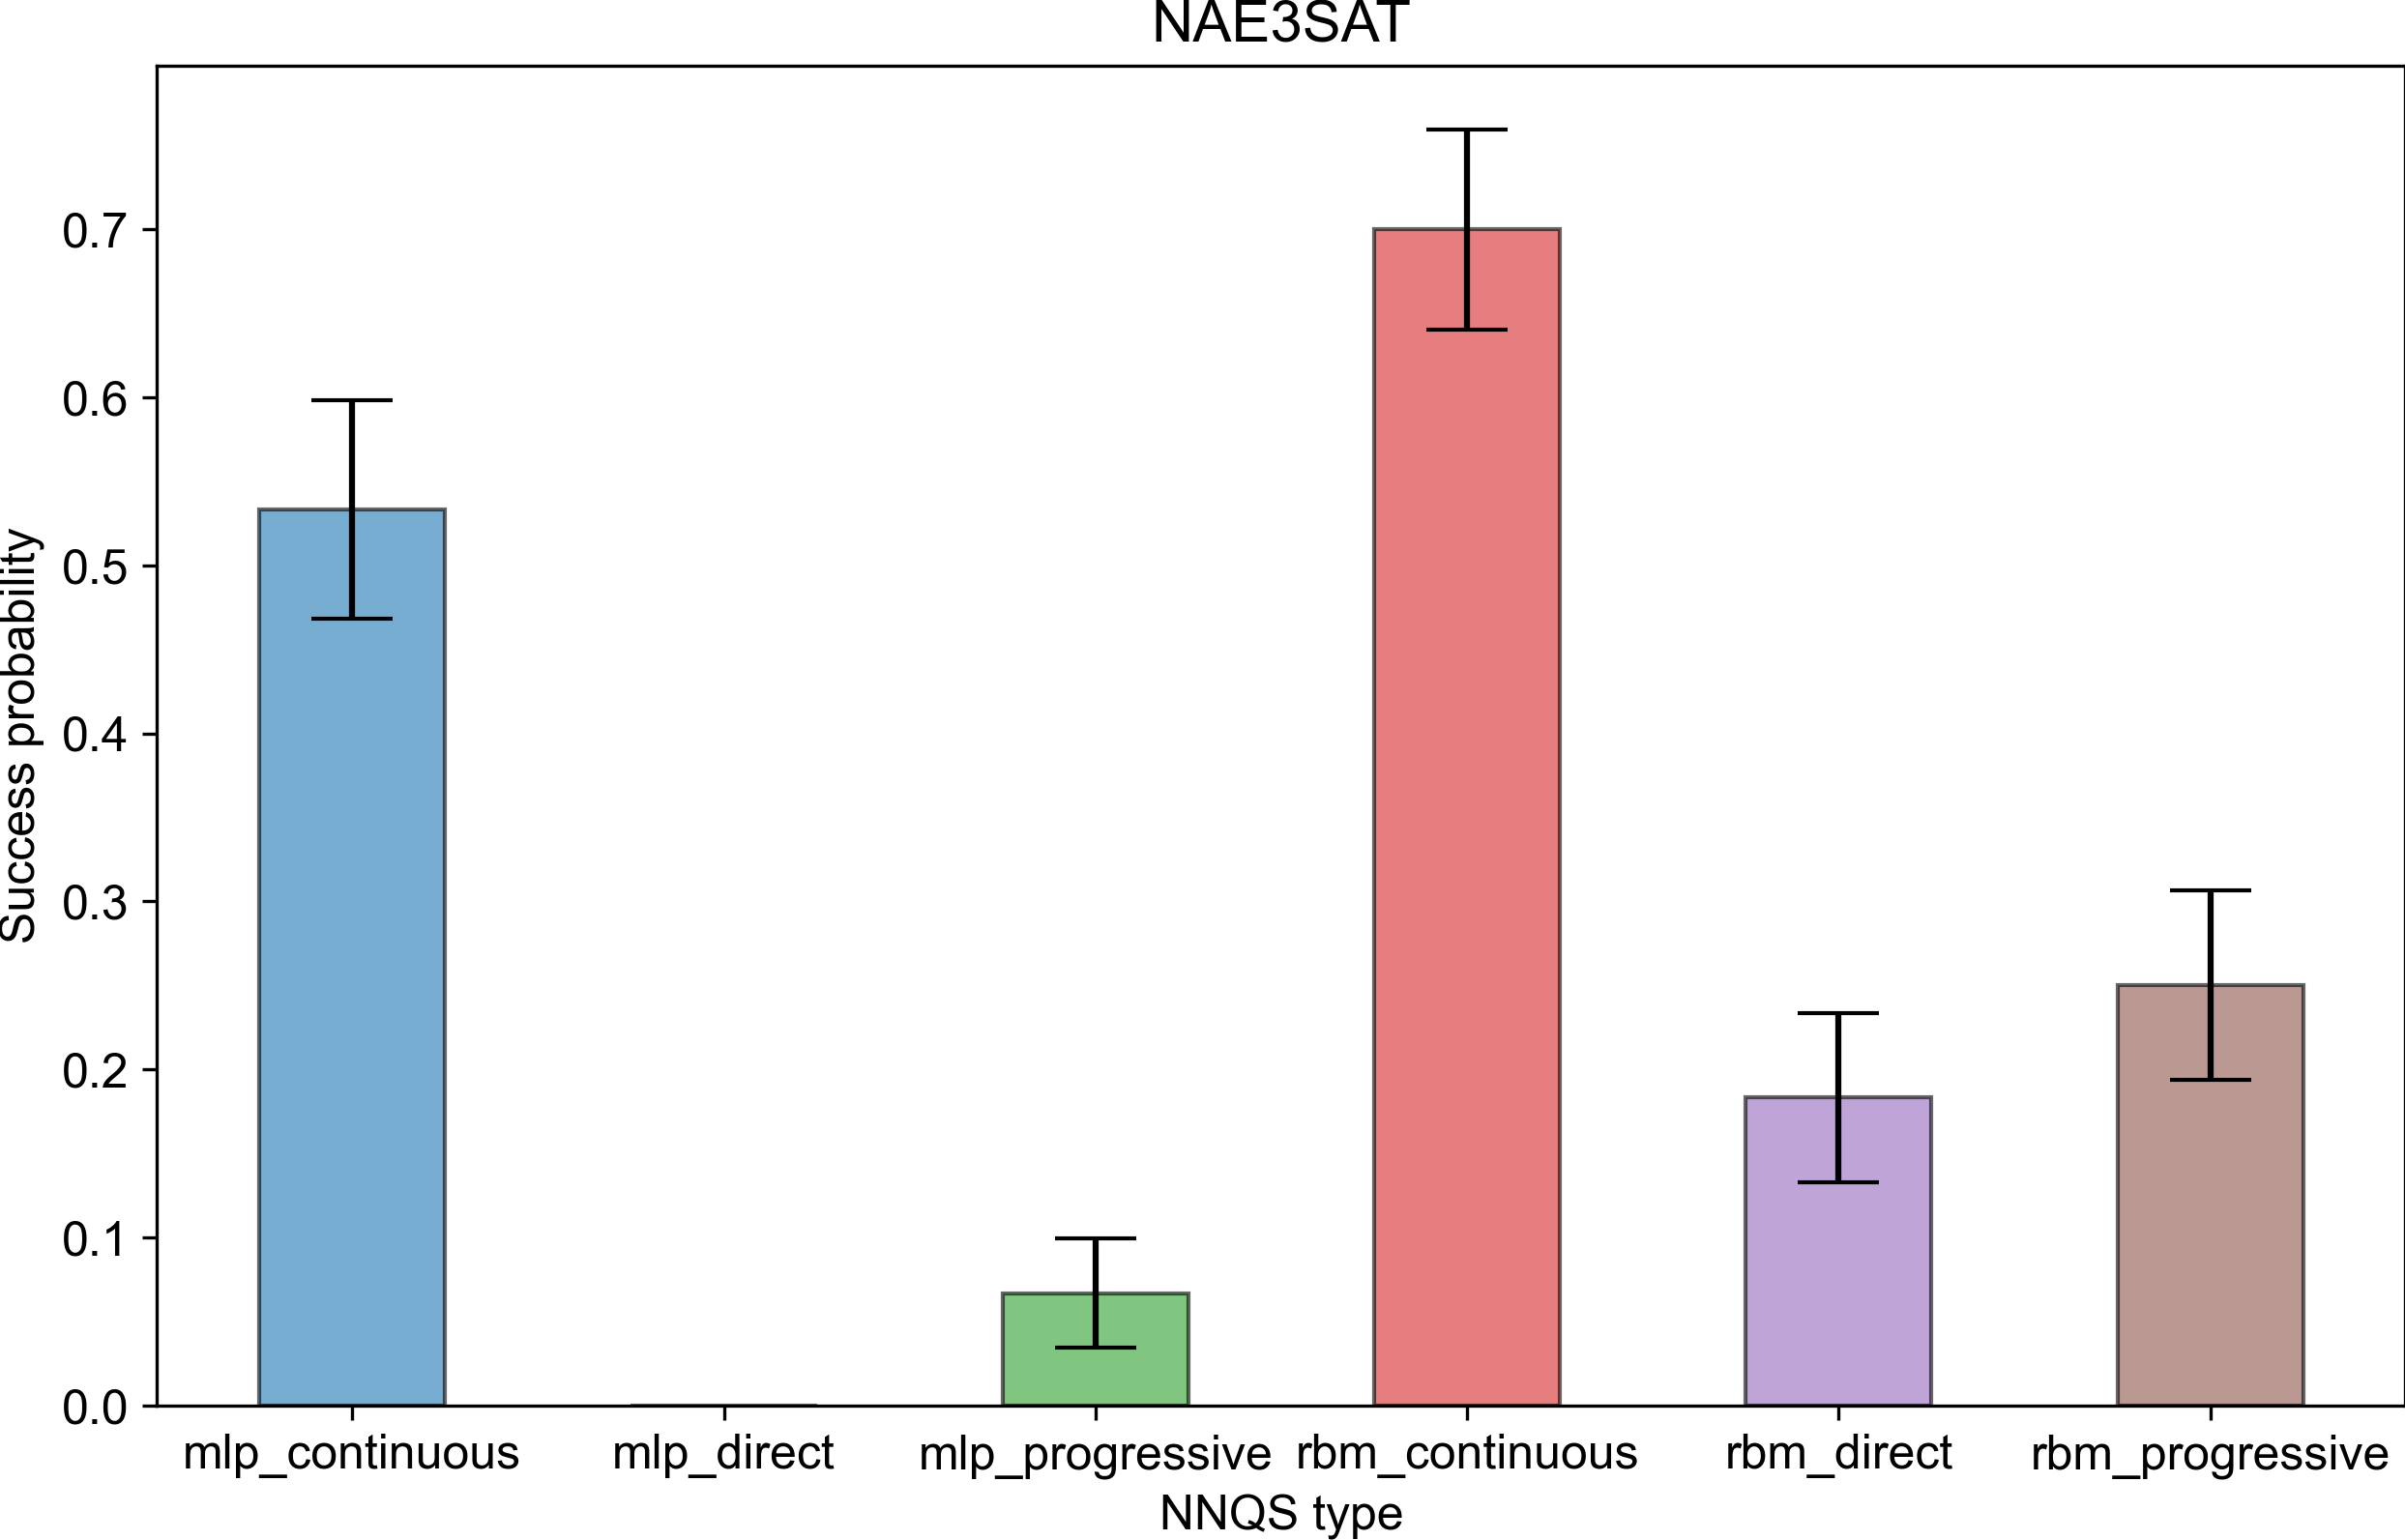
\includegraphics[width=0.49\textwidth]{images/nae3sat_nnqs_success_avg.png}}
    \caption{Average performance of different NNQS types for NAE3SAT}
    \label{nnqs-nae3sat-average}
\end{figure}

For the NAE3SAT dataset, the continuous training algorithm with the RBM performs the best in average performance and success probability when averaged across all sizes, shown in \autoref{nnqs-nae3sat-average}. In the performance by problem size, the continuous training algorithm with the RBM performed the best in normalised energy and success probability, shown in \autoref{nnqs-nae3sat-size}, except with a problem size of $50$, which is likely due to variance in the randomly generated data set. 

\subsection{Max-cut}

\begin{figure}[!htbp]
    \centering
    \subfloat[Normalized energy]{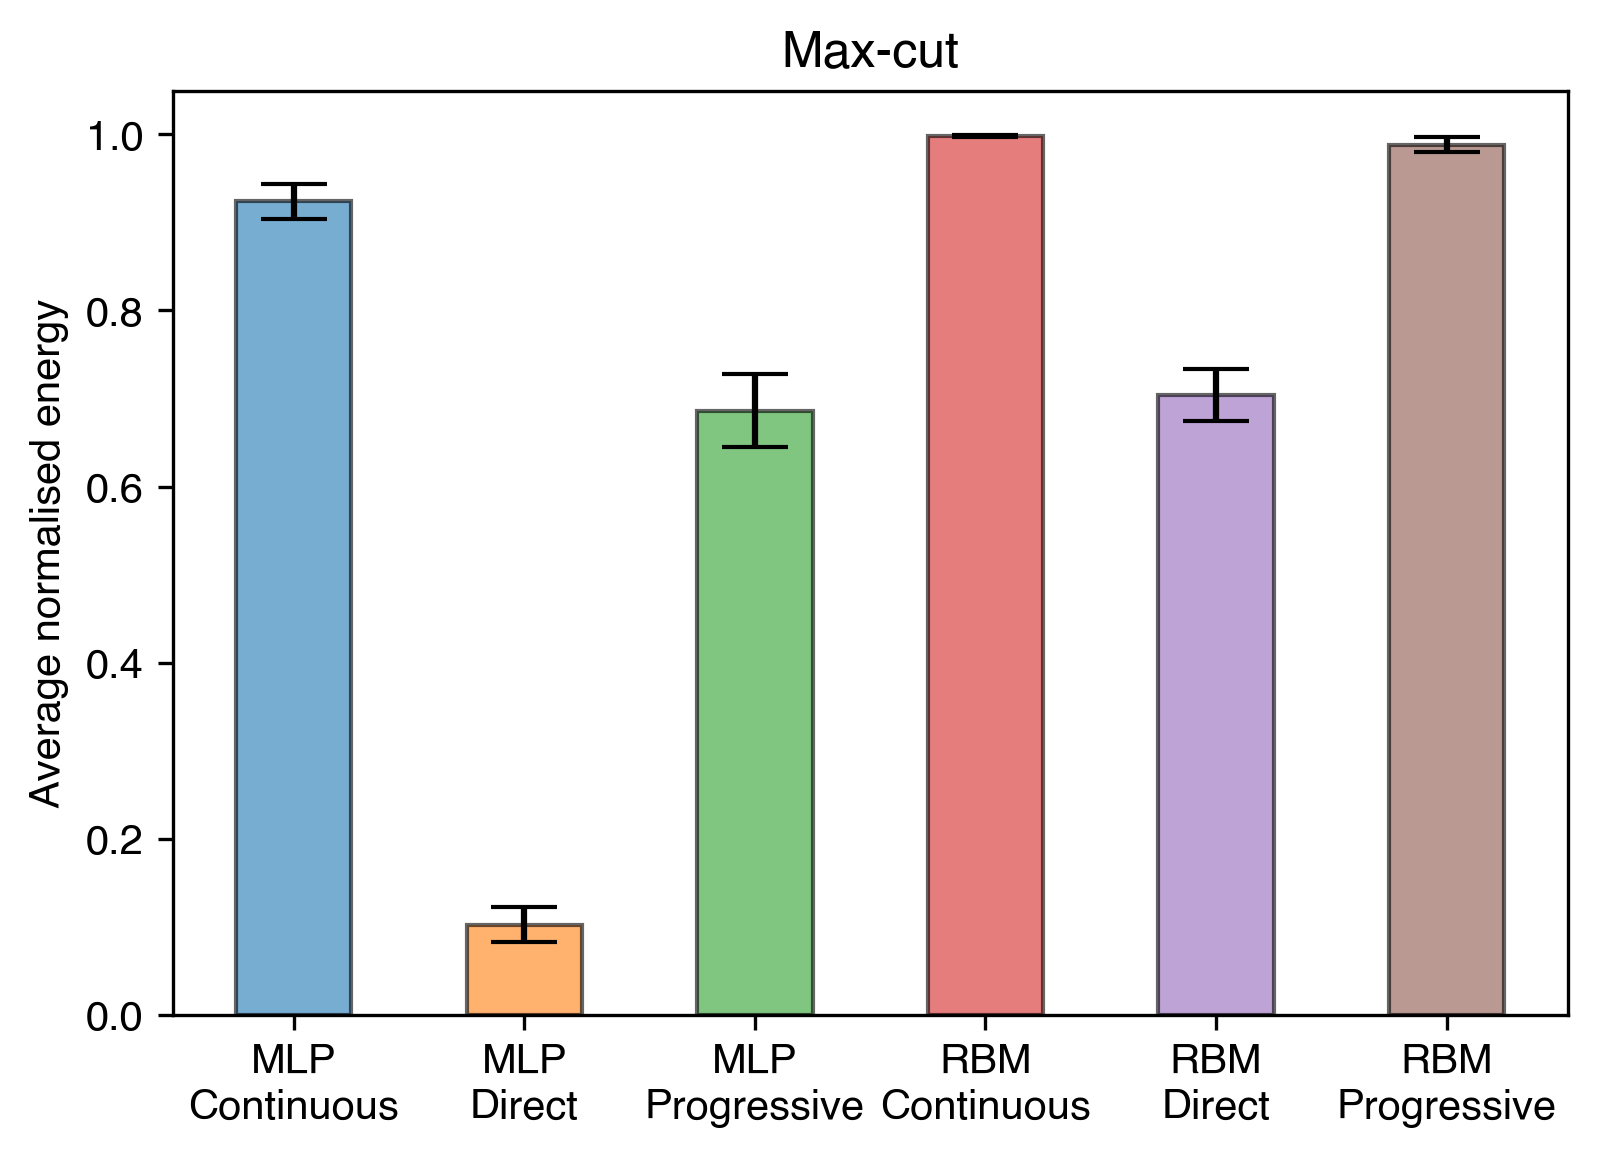
\includegraphics[width=0.49\textwidth]{images/maxcut_nnqs_avg.png}}\hfill
    \subfloat[Success probability]{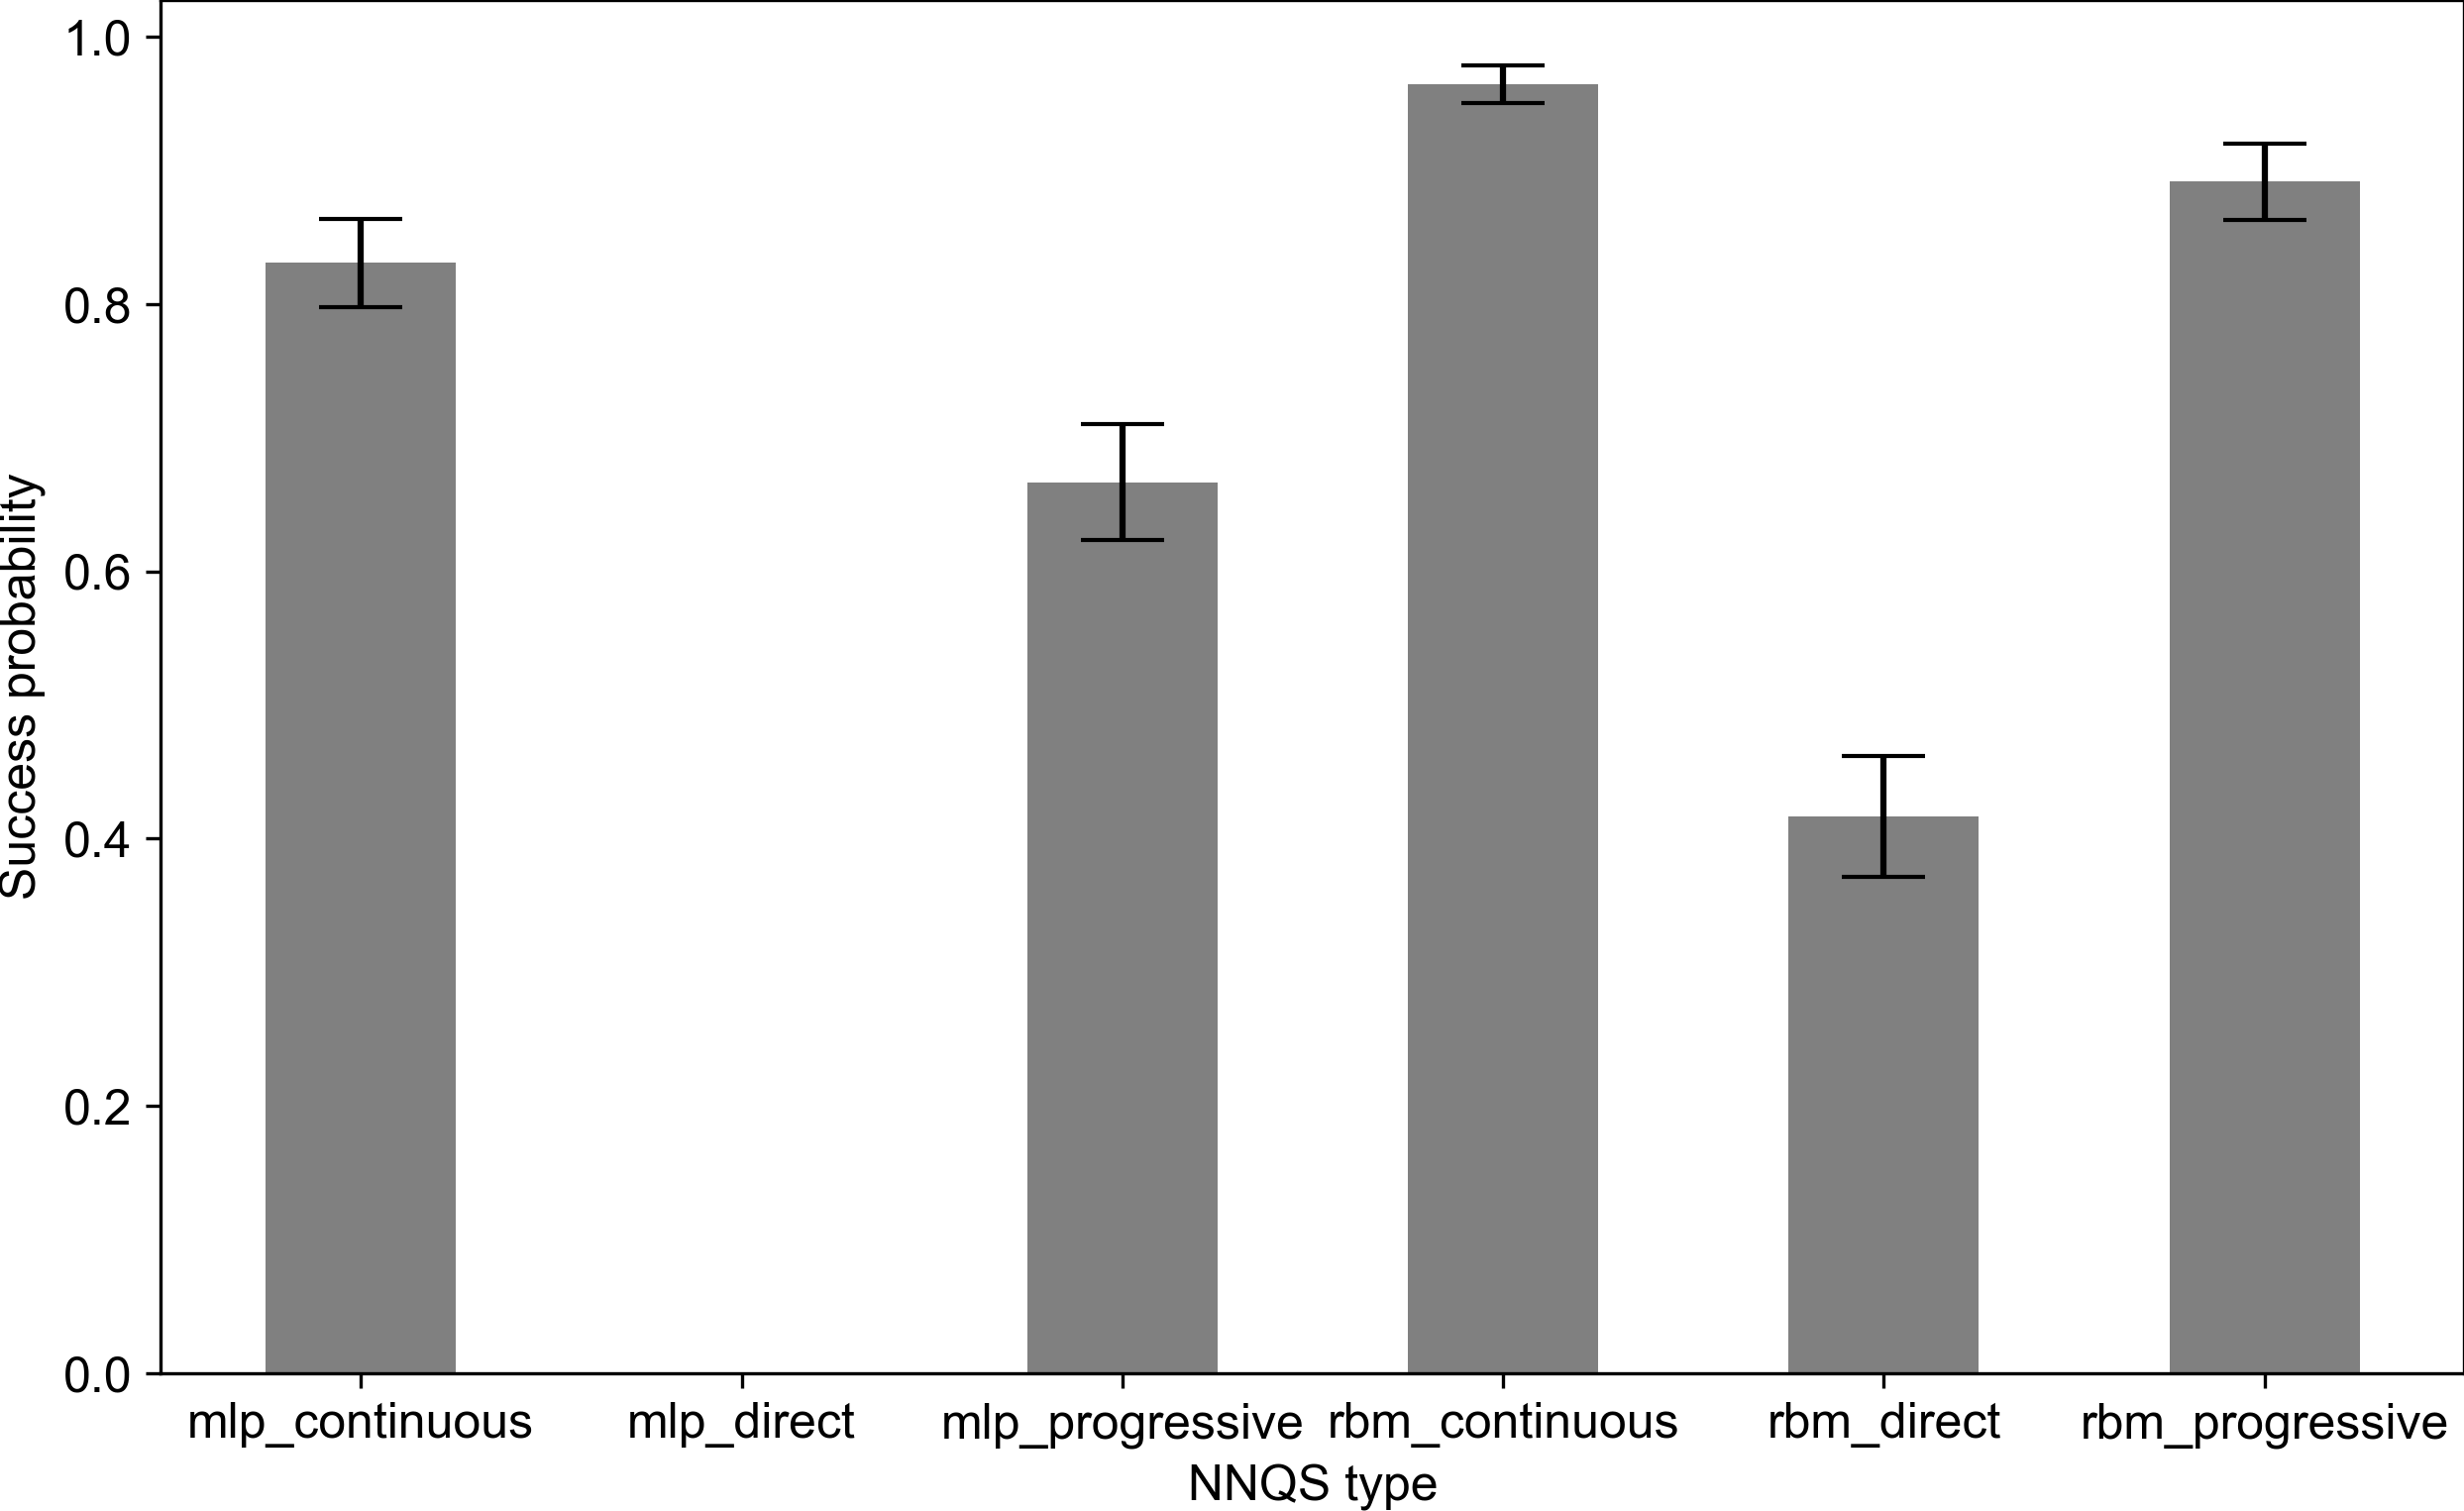
\includegraphics[width=0.49\textwidth]{images/maxcut_nnqs_success_avg.png}}
    \caption{Average performance of different NNQS types for max-cut}
    \label{nnqs-maxcut-average}
\end{figure}

For the maxcut dataset, the continuous training algorithm with the RBM performs the best in average performance and success probability when averaged across all sizes, shown in \autoref{nnqs-maxcut-average}. In the performance by problem size, the continuous training algorithm with the RBM performed the best in normalised energy and success probability, shown in \autoref{nnqs-maxcut-size}, except with a problem size of $25$, which is again likely due to variance in the randomly generated data set. However, the gap in success probability between the models is relatively small, which likely implies that the max-cut problem is easier in general than the NAE3SAT problem.


\subsection{SK model}

\begin{figure}[!htbp]
    \centering
    \subfloat[Normalized energy]{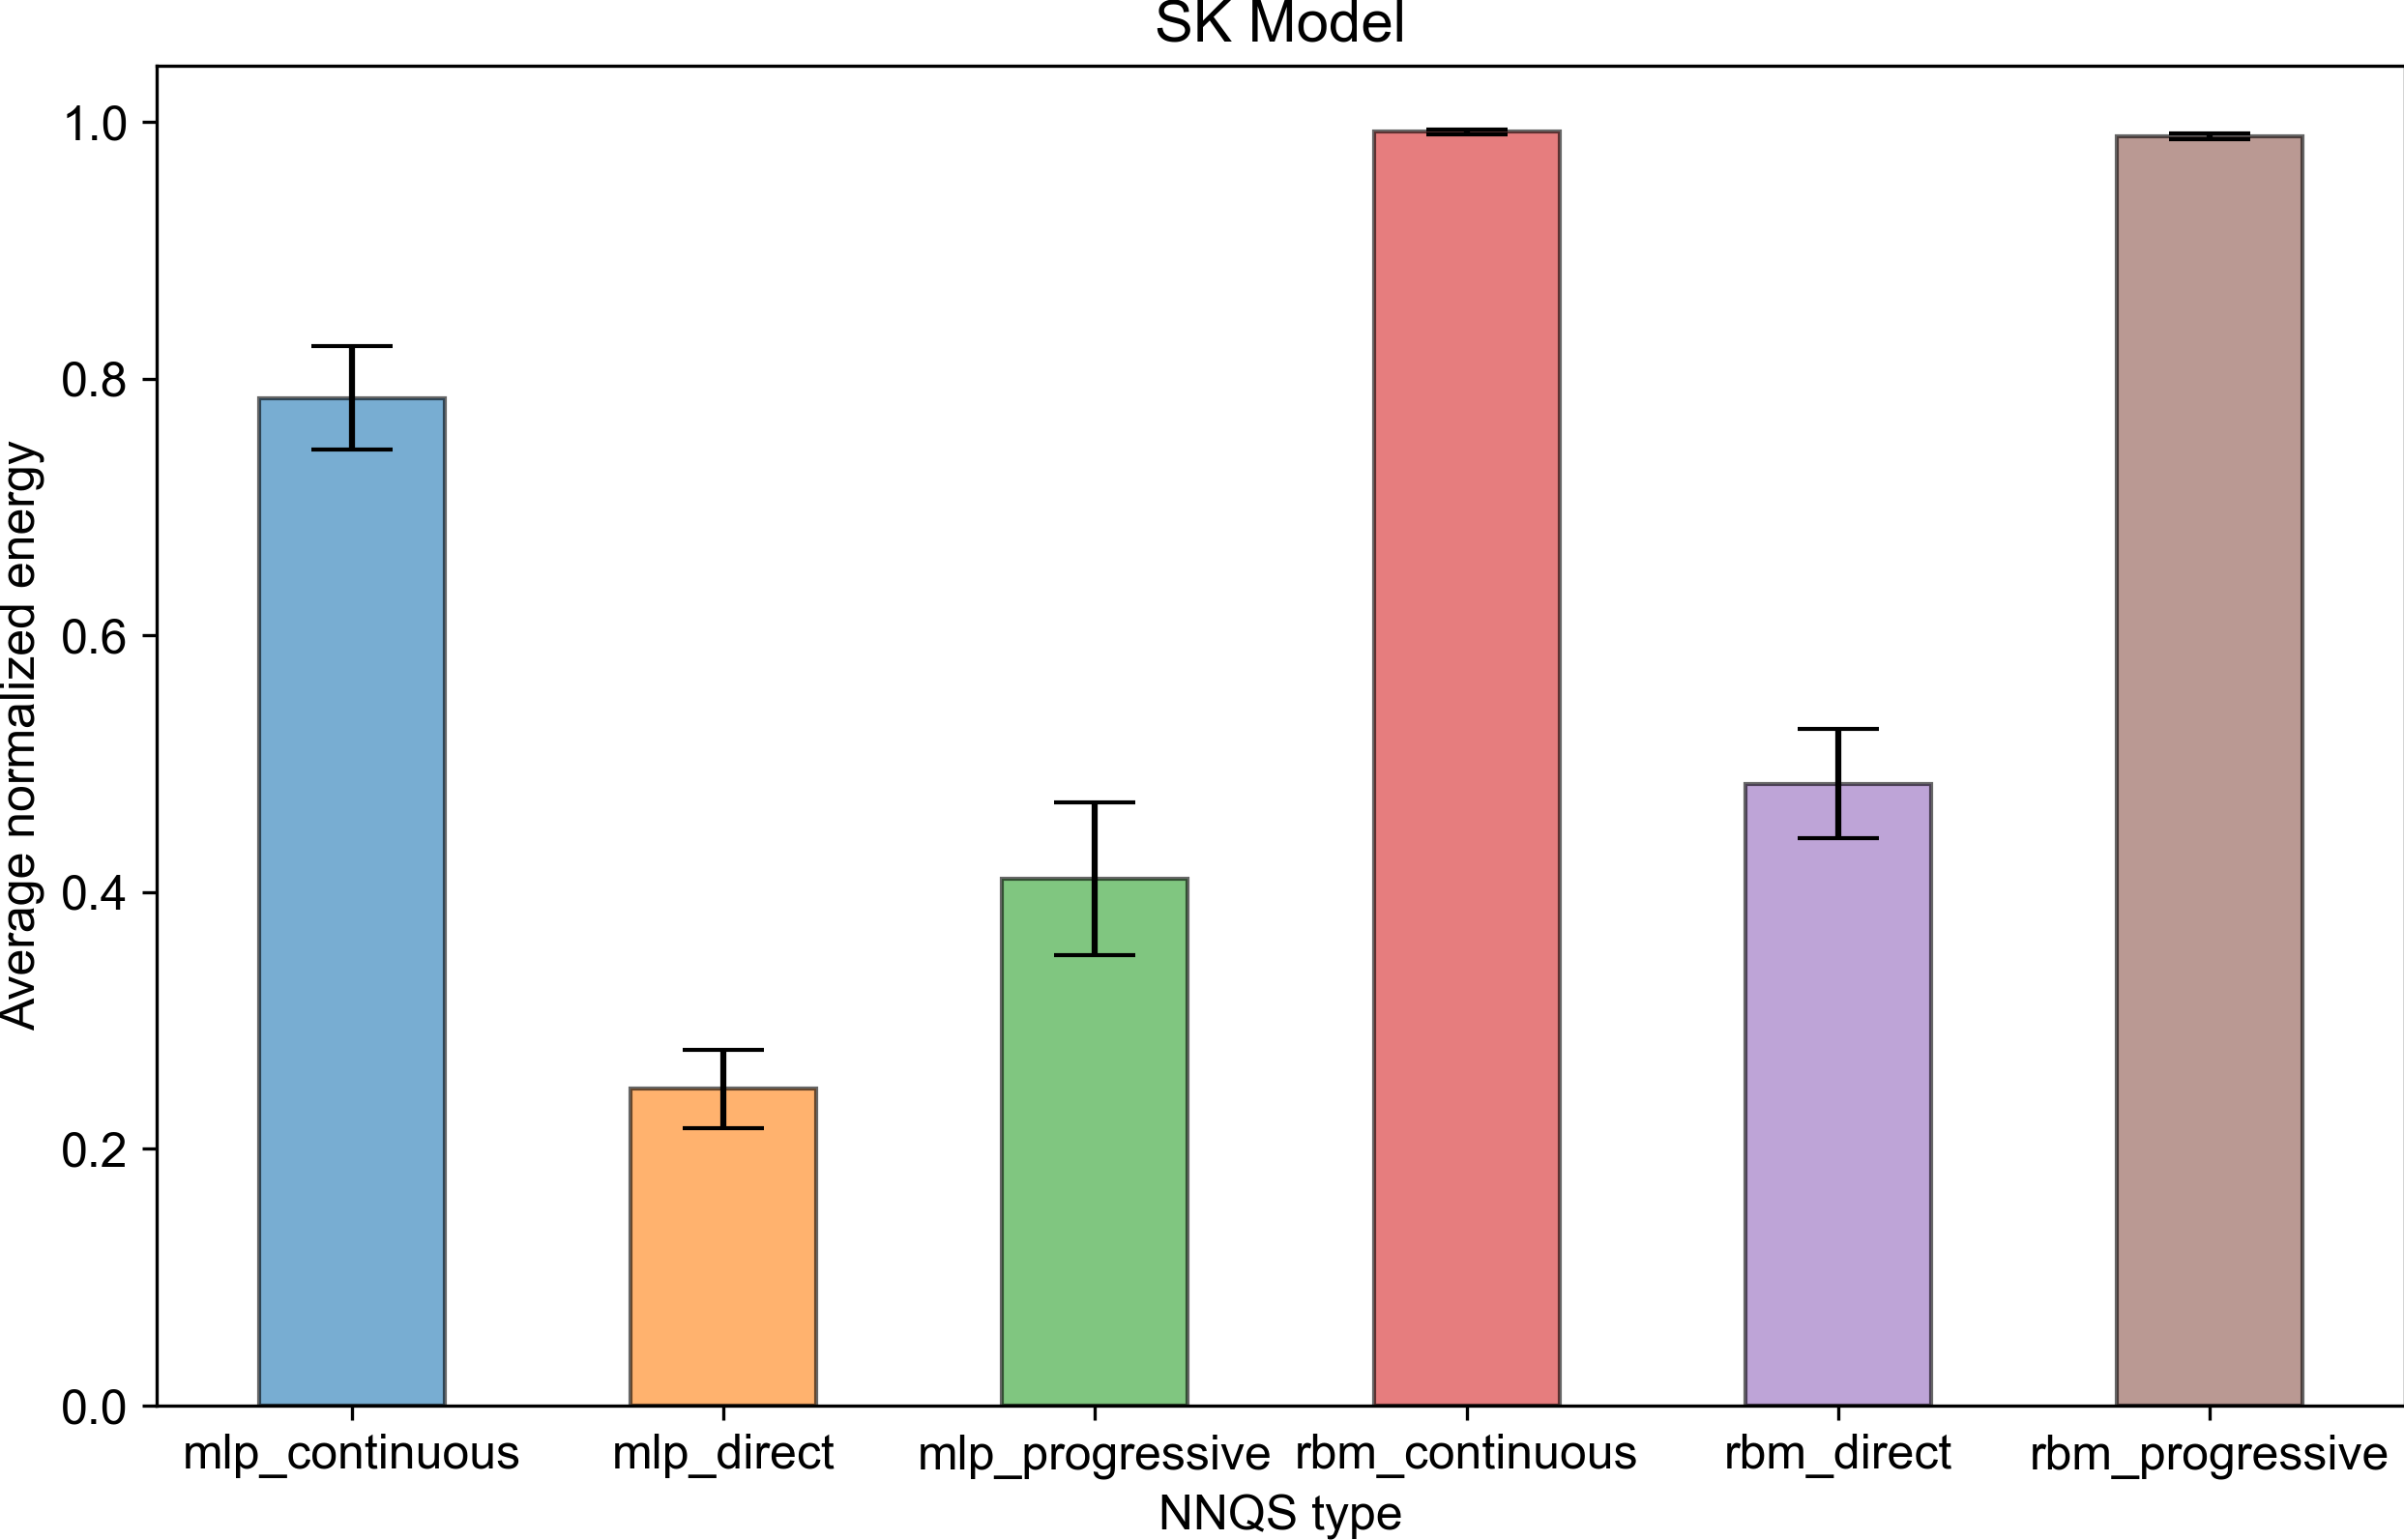
\includegraphics[width=0.49\textwidth]{images/skmodel_nnqs_avg.png}}\hfill
    \subfloat[Success probability]{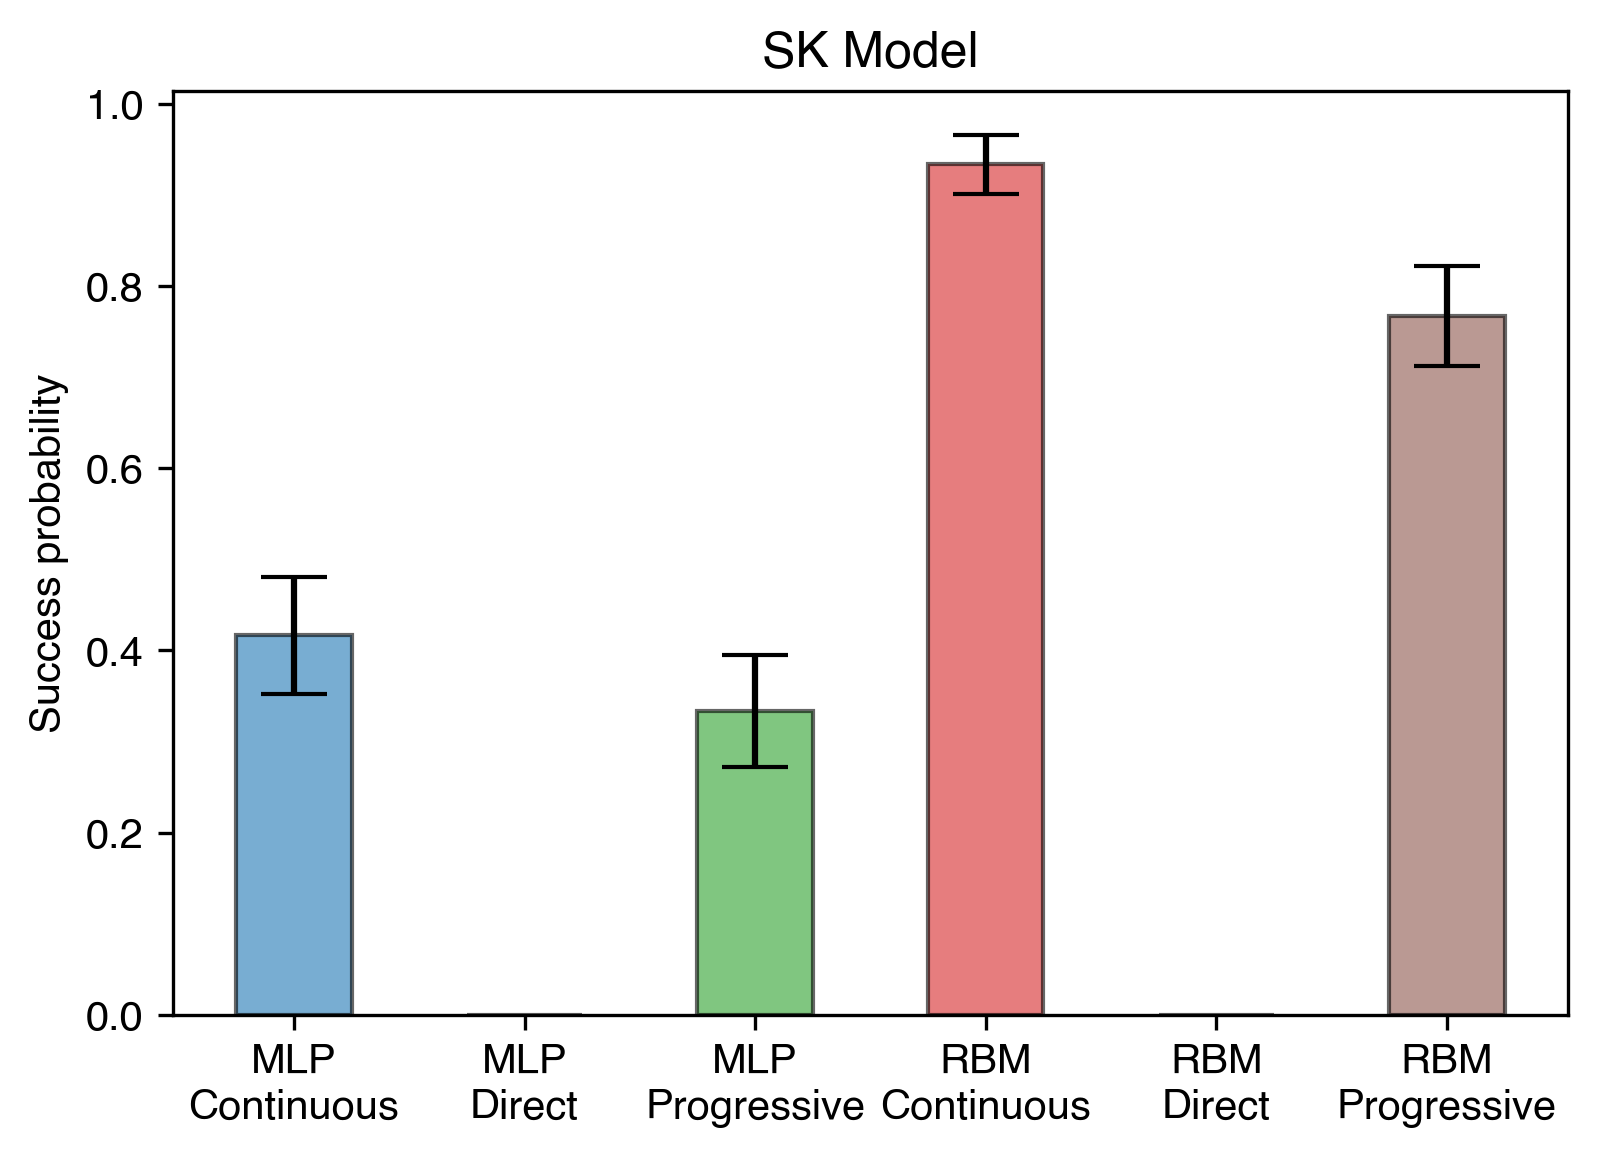
\includegraphics[width=0.49\textwidth]{images/skmodel_nnqs_success_avg.png}}
    \caption{Average performance of different NNQS types for SK model}
    \label{nnqs-skmodel-average}
\end{figure}

For the SK model dataset, the continuous training algorithm with the RBM performs the best in average performance and success probability when averaged across all sizes, shown in \autoref{nnqs-skmodel-average}. The performance averaged across all sizes, shown in \autoref{nnqs-skmodel-average}, also highlights that the RBM with a continuous training algorithm performs the best. However, it is interesting that the direct training schemes perform poorly with small problem sizes ($\leq 50$) but are relatively better at higher problem sizes ($100, 250$).

\section{Conclusion}
\autoref{results:nnqsnormalizedenergy} and \autoref{results:nnqssuccess} show the average normalised energy and success probability for different types of NNQS for each dataset and the average across all datasets.

Across all the problem sets, the RBM has a better average performance than the MLP in average normalised energy and success probability for each training algorithm. In terms of training schemes, direct training performs the worst among the 3, and continuous training performs slightly better than progressive training. Using the RBM with a continuous training scheme gives the highest normalised energy and success probability across all datasets. 

Even though progressive training more closely mimics the quantum annealing process in D-wave solvers, the sudden change of Hamiltonian may have led to large gradient changes that may have made it more difficult for the network to converge, leading to poorer training. Continuous training gradually changes the Hamiltonian, which limits the gradient magnitudes and may result in better training. Direct training is expected to have poor performance as it tends to get stuck in local minima.


\begin{table}[!ht]
    \centering
    \begin{tabular}{ccccccc} \toprule
        ~ & \multicolumn{3}{c}{MLP} & \multicolumn{3}{c}{RBM} \\
        \cmidrule{2-7} & Continuous & Direct & Progressive & Continuous & Direct & Progressive \\
        \midrule
        NAE3SAT & 0.866 & 0.118 & 0.352 & \textbf{0.997} & 0.511 & 0.910 \\
        Max-cut & 0.924 & 0.102 & 0.686 & \textbf{0.998} & 0.704 & 0.988 \\
        SK model & 0.790 & 0.248 & 0.411 & \textbf{0.999} & 0.488 & 0.995 \\ \midrule
        Average & 0.860 & 0.156 & 0.483 & \textbf{0.998} & 0.568 & 0.965 \\ \bottomrule
    \end{tabular}
    \caption{Average normalised energy for different NNQS types}
    \label{results:nnqsnormalizedenergy}
\end{table}

\begin{table}[!ht]
    \centering
    \begin{tabular}{ccccccc} \toprule
        ~ & \multicolumn{3}{c}{MLP} & \multicolumn{3}{c}{RBM} \\
        \cmidrule{2-7} & Continuous & Direct & Progressive & Continuous & Direct & Progressive \\
        \midrule
        NAE3SAT & 0.583 & 0.029 & 0.062 & \textbf{0.950} & 0.167 & 0.364 \\
        Max-cut & 0.831 & 0.000 & 0.667 & \textbf{0.965} & 0.417 & 0.892 \\
        SK model & 0.417 & 0.000 & 0.333 & \textbf{0.933} & 0.000 & 0.767 \\ \midrule
        Average & 0.610 & 0.010 & 0.354 & \textbf{0.949} & 0.194 & 0.674 \\ \bottomrule
    \end{tabular}
    \caption{Success probability for different NNQS types}
    \label{results:nnqssuccess}
\end{table}